\chapter{模板(Stenciling)}
\begin{flushleft}
模板缓冲区是一个屏幕外缓冲区,我们可以使用它来实现一些特殊效果。 模板缓冲区具有与后缓冲区和深度缓冲区相同的分辨率,使得模板缓冲区中的第$i$个像素对应于后缓冲区和深度缓冲区中的第$i$个像素。 回想一下4.1.5,当指定模板缓冲区时,它会附加到深度缓冲区。 顾名思义,模板缓冲区用作模板,允许我们阻止某些像素片段渲染到后台缓冲区。\\

例如,在实现镜像时,我们需要在镜子的平面上反射一个物体; 但是,我们只想将反射绘制到镜子中。 我们可以使用模板缓冲区来阻止反射的渲染,除非它被绘制到镜像中(见图\ref{fig:11-1})。
\end{flushleft}

\begin{figure}[h]
    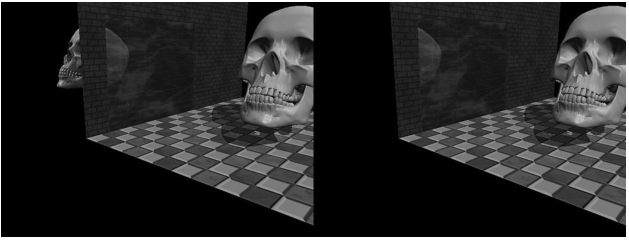
\includegraphics[width=\textwidth]{11-1}
    \centering
    \caption{(左)反射的头骨在镜子中正确显示。 墙体砖没有显示反射,因为它未能在该区域进行深度测试。 然而,在墙后面看,我们能够看到反射,从而打破了幻像(反射应该只通过镜子出现)。 (右)通过使用模板缓冲区,我们可以阻止反射的头骨被渲染,除非它被绘制在镜子中。}
    \label{fig:11-1}
\end{figure}

\begin{flushleft}
通过填写 D3D12\_DEPTH\_STENCIL\_DESC 实例并将其分配给管道状态对象(PSO)的 D3D12\_GRAPHICS\_PIPELINE\_STATE\_DESC::DepthStencilState 字段来配置模板缓冲区(以及深度缓冲区)状态。 通过研究现有的示例应用程序,学习有效地使用模板缓冲区。 一旦您了解了模板缓冲区的一些应用程序,您就可以更好地了解它如何用于您自己的特定需求。
{\large Objectives:}
\begin{itemize}
    \item 1.通过填写管道状态对象中的 D3D12\_DEPTH\_STENCIL\_DESC 字段来了解如何控制深度和模板缓冲区状态。
    \item 2.了解如何通过使用模板缓冲区来实现镜像,以防止反射被绘制到非镜像表面。
    \item 3.能够识别双重混合并理解模板缓冲区是如何防止它的。
    \item 4.解释深度复杂性,描述两种可以测量场景的深度复杂度的方式。
\end{itemize}
\end{flushleft}

%-------- 11.1 --------
\section{深度/模板格式和清除(Depth/Stencil Formats and Clearing)}
\begin{flushleft}
回忆深度/模板缓冲区是一种纹理,必须使用某些数据格式创建。用于深度/模板缓冲的格式如下:\\
\end{flushleft}

\begin{itemize}
  \item 1.DXGI\_FORMAT\_D32\_FLOAT\_S8X24\_UINT: 指定一个32位浮点型深度缓冲区,保留8位(无符号整数)用于映射到$[0,255]$范围的模板缓冲区,剩余24位不用于填充。
  \item 2.DXGI\_FORMAT\_D24\_UNORM\_S8\_UINT: 指定映射到$[0,1]$范围的无符号24位深度缓冲区,其中8位(无符号整数)保留给映射到$[0,255]$范围的模板缓冲区。
\end{itemize}

\begin{flushleft}
在我们的D3DApp框架中,当创建深度缓冲区时,指定:\\
\end{flushleft}

\begin{lstlisting}
DXGI_FORMAT mDepthStencilFormat = DXGI_FORMAT_D24_UNORM_S8_UINT;
depthStencilDesc.Format = mDepthStencilFormat;
\end{lstlisting}

\begin{flushleft}
此外,模板缓冲区应在每帧开始时重置为某个值。这是通过以下方法完成的(它也清除了深度缓冲区):\\
\end{flushleft}

\begin{lstlisting}
void ID3D12GraphicsCommandList::ClearDepthStencilView(
    D3D12_CPU_DESCRIPTOR_HANDLE DepthStencilView,
    D3D12_CLEAR_FLAGS ClearFlags,
    FLOAT Depth,
    UINT8 Stencil,
    UINT NumRects,
    const D3D12_RECT *pRects);
\end{lstlisting}

\begin{flushleft}
1.DepthStencilView: 我们想要清除深度/模板缓冲区视图的描述符。\\

2.ClearFlags: 指定 D3D12\_CLEAR\_FLAG\_DEPTH 仅清除深度缓冲区; 指定 D3D12\_CLEAR\_FLAG\_STENCIL 仅清除模板缓冲区; 指定 D3D12\_CLEAR\_FLAG\_DEPTH | D3D12\_CLEAR\_FLAG\_STENCIL 清除两者。\\

3.Depth: float-value 用于设置深度缓冲区中的每个像素; 它必须是浮点数$x$,$0\leq x\leq 1$。\\

4.Stencil: 用于设置模板缓冲区的每个像素的整数值; 它必须是整数$n$,$0\leq n\leq 255$。\\

5.NumRects: pRects指向的数组中的矩形数。\\

6.pRects: D3D12\_RECT 数组,用于标记深度/模板缓冲区上的矩形区域以进行清除; 指定 nullptr 以清除整个深度/模板缓冲区。\\
~\\
我们已经在演示的每个帧中调用了这个方法。:\\
mCommandList->ClearDepthStencilView(
    DepthStencilView(),
    D3D12_CLEAR_FLAG_DEPTH | D3D12_CLEAR_FLAG_STENCIL,
    1.0f, 0, 0, nullptr);
\end{flushleft}

%-------- 11.2 --------
\section{模板测试(The Stencil Test)}
\begin{flushleft}
如前所述,我们可以使用模板缓冲区来阻止渲染到后缓冲区的某些区域。 阻止特定像素被写入由模板测试决定,模板测试由以下内容给出:\\
\end{flushleft}

\begin{lstlisting}
if( StencilRef 
    & StencilReadMask Value 
    & StencilReadMask )
    accept pixel
else
    reject pixel
\end{lstlisting}

\begin{flushleft}
当像素被光栅化时(即,在输出合并阶段期间)执行模板测试,假设启用了模板,并采用两个操作数:\\

1.左侧(left-hand-side LHS)操作数,通过将应用程序定义的模板参考值(StencilRef)与应用程序定义的屏蔽值(StencilReadMask)进行AND运算确定。\\

2.右侧(right-hand-side RHS)操作数,通过对已经在模板缓冲区中的特定像素测试值(Value)与应用程序定义的屏蔽值(StencilReadMask)进行AND运算来确定。\\
~\\
请注意,LHS和RHS的StencilReadMask是相同的。 然后,模板测试将LHS与RHS进行比较,指定应用程序选择的比较函数,该函数返回true或false值。 如果测试结果为true,我们将像素写入后缓冲区(假设深度测试也通过)。 如果测试结果为false,那么我们阻止将像素写入后缓冲区。 当然,如果由于模板测试失败而导致像素被拒绝,则也不会将其写入深度缓冲区。\\

$\unlhd$操作符含义由下面枚举类定义:\\
\end{flushleft}

\begin{lstlisting}
typedef enum D3D12_COMPARISON_FUNC
{
    D3D12_COMPARISON_NEVER = 1,
    D3D12_COMPARISON_LESS = 2,
    D3D12_COMPARISON_EQUAL = 3,
    D3D12_COMPARISON_LESS_EQUAL = 4,
    D3D12_COMPARISON_GREATER = 5,
    D3D12_COMPARISON_NOT_EQUAL = 6,
    D3D12_COMPARISON_GREATER_EQUAL = 7,
    D3D12_COMPARISON_ALWAYS = 8,
} D3D12_COMPARISON_FUNC;
\end{lstlisting}
\begin{itemize}
  \item 1.D3D12\_COMPARISON\_NEVER:函数总是返回 false。
  \item 2.D3D12\_COMPARISON\_LESS:替换$\unlhd$为 $<$符号。
  \item 3.D3D12\_COMPARISON\_EQUAL:替换$\unlhd$为 $==$符号。
  \item 4.D3D12\_COMPARISON\_LESS\_EQUAL:替换$\unlhd$为 $\leq$符号。
  \item 5.D3D12\_COMPARISON\_GREATER:替换$\unlhd$为 $>$符号。
  \item 6.D3D12\_COMPARISON\_NOT\_EQUAL:替换$\unlhd$为 $!=$符号。
  \item 7.D3D12\_COMPARISON\_GREATER\_EQUAL:替换$\unlhd$为 $\geq$符号。
  \item 8.D3D12\_COMPARISON\_ALWAYS:函数总是返回 true。
\end{itemize}

%-------- 11.3 --------
\section{描述深度/模板状态(Describing The Depth/Stencil State)}
\begin{flushleft}
深度/模板状态由 D3D12\_DEPTH\_STENCIL\_DESC 实例填充定义:\\ 
\end{flushleft}

\begin{lstlisting}
typedef struct D3D12_DEPTH_STENCIL_DESC {
    BOOL DepthEnable; // Default True
    // Default: D3D11_DEPTH_WRITE_MASK_ALL
     D3D12_DEPTH_WRITE_MASK DepthWriteMask;
    // Default: D3D11_COMPARISON_LESS
    D3D12_COMPARISON_FUNC DepthFunc;
    BOOL StencilEnable; // Default: False
    UINT8 StencilReadMask; // Default: 0xff
    UINT8 StencilWriteMask; // Default: 0xff
    D3D12_DEPTH_STENCILOP_DESC FrontFace;
    D3D12_DEPTH_STENCILOP_DESC BackFace;
} D3D12_DEPTH_STENCIL_DESC;
\end{lstlisting}

%-------- 11.3.1 --------
\subsection{深度设置(Depth Settings)}
\begin{flushleft}
1.DepthEnable: 指定true以启用深度缓冲; 指定false以禁用它。 禁用深度测试时,绘制顺序很重要,即使它位于遮挡对象后面,也会绘制像素片段(回顾4.1.5)。 如果禁用深度缓冲,则无论DepthWriteMask设置如何,深度缓冲区中的元素也不会更新。\\

2.DepthWriteMask: 这可以是 D3D12\_DEPTH\_WRITE\_MASK\_ZERO 或 D3D12\_DEPTH\_WRITE\_MASK\_ALL,但不能同时使用两者。假设 DepthEnable 设置为 true,D3D12\_DEPTH\_WRITE\_MASK\_ZERO禁用对深度缓冲区的写入,但仍会进行深度测试。D3D12\_DEPTH\_WRITE\_MASK\_ALL允许写入深度缓冲区; 如果深度和模板测试都通过,将写入新的深度。 控制深度读取和写入的能力对于实现某些特殊效果是必要的。\\

3.DepthFunc: 指定 D3D12\_COMPARISON\_FUNC 枚举类型的成员之一以定义深度测试比较功能。 通常这总是 D3D12\_COMPARISON\_LESS,以便执行通常的深度测试,如4.1.5中所述。 也就是说,如果像素片段的深度值小于写入后缓冲器的前一像素的深度,则接受该像素片段。 但正如您所看到的,Direct3D允许您在必要时自定义深度测试。\\
\end{flushleft}

%-------- 11.3.2 --------
\subsection{模板设置(Stencil Settings)}
\begin{flushleft}
1.StencilEnable: 指定 true 以启用模板测试; 指定 false 以禁用它。\\
2.StencilReadMask: StencilReadMask 在模板测试时使用:\\
\end{flushleft}

\begin{lstlisting}
if( StencilRef 
    & StencilReadMask Value 
    & StencilReadMask )
    accept pixel
else
    reject pixel
\end{lstlisting}

\begin{flushleft}
默认值不屏蔽任何位:\\
\end{flushleft}
\begin{lstlisting}
#define D3D12_DEFAULT_STENCIL_READ_MASK (0xff)
\end{lstlisting}

\begin{flushleft}
3.StencilWriteMask: 当更新模板缓冲区时,我们可以使用写掩码(Write Mask)屏蔽掉某些位。 例如,如果要阻止写入前4位,可以使用 0x0f 的写掩码。 默认值不会屏蔽任何位:\\
\end{flushleft}
\begin{lstlisting}
#define D3D12_DEFAULT_STENCIL_WRITE_MASK (0xff)
\end{lstlisting}

\begin{flushleft}
4.FrontFace: 填写 D3D12\_DEPTH\_STENCILOP\_DESC 结构,指示模板缓冲区如何对前置三角形起作用。\\

5.BackFace: 填写 D3D12\_DEPTH\_STENCILOP\_DESC 结构,指示模板缓冲区如何对后置三角形起作用。\\
\end{flushleft}

\begin{lstlisting}
typedef struct D3D12_DEPTH_STENCILOP_DESC {
    D3D12_STENCIL_OP StencilFailOp; // Default: D3D12_STENCIL_OP_KEEP
    D3D12_STENCIL_OP StencilDepthFailOp; // Default: D3D12_STENCIL_OP_KEEP
    D3D12_STENCIL_OP StencilPassOp; // Default: D3D12_STENCIL_OP_KEEP
    D3D12_COMPARISON_FUNC StencilFunc; // Default: D3D12_COMPARISON_ALWAYS
} D3D12_DEPTH_STENCILOP_DESC;
\end{lstlisting}

\begin{flushleft}
(1).StencilFailOp: D3D12\_STENCIL\_OP 枚举类型的成员,描述当像素片段的模板测试失败时应如何更新模板缓冲区。\\
(2).StencilDepthFailOp: D3D12\_STENCIL\_OP 枚举类型的成员,描述在像素片段的模板测试通过然而深度测试失败时如何更新模板缓冲区。\\
(3).StencilPassOp: D3D12\_STENCIL\_OP 枚举类型的成员,描述当像素片段的模板测试和深度测试都通过时应如何更新模板缓冲区。\\
(4).StencilFunc: D3D12\_COMPARISON\_FUNC 枚举类型的成员,用于定义模板测试比较函数。
\end{flushleft}

\begin{lstlisting}
typedef enum D3D12_STENCIL_OP
{
    D3D12_STENCIL_OP_KEEP = 1,
    D3D12_STENCIL_OP_ZERO = 2,
    D3D12_STENCIL_OP_REPLACE = 3,
    D3D12_STENCIL_OP_INCR_SAT = 4,
    D3D12_STENCIL_OP_DECR_SAT = 5,
    D3D12_STENCIL_OP_INVERT = 6,
    D3D12_STENCIL_OP_INCR = 7,
    D3D12_STENCIL_OP_DECR = 8
} D3D12_STENCIL_OP;
\end{lstlisting}

\begin{flushleft}
(1).D3D12\_STENCIL\_OP\_KEEP: 指定不更改模板缓冲区; 也就是说,保持当前的值。\\
(2).D3D12\_STENCIL\_OP\_ZERO: 指定将模板缓冲区条目设置为零。\\
(3).D3D12\_STENCIL\_OP\_REPLACE: 指定使用模板测试中使用的模板参考值(StencilRef)替换模板缓冲区条目。 请注意,当我们将深度/模板状态块绑定到渲染管道(第11.3.3节)时,会设置 StencilRef 值。\\
(4).D3D12\_STENCIL\_OP\_INCR\_SAT:指定增加模板缓冲区条目。 如果递增的值超过最大值(例如,对于8位模板缓冲区为255),则我们将条目钳位到该最大值。\\
(5).D3D12\_STENCIL\_OP\_DECR\_SAT:指定递减模板缓冲区条目。 如果递减的值小于零,那么我们将条目钳位为零。\\
(6).D3D12\_STENCIL\_OP\_INVERT:指定反转模板缓冲区条目的位。\\
(7).D3D12\_STENCIL\_OP\_INCR: 指定增加模板缓冲区条目。 如果递增的值超过最大值(例如,对于8位模板缓冲区为255),则我们将其换行为0。\\
(8).D3D12\_STENCIL\_OP\_DECR: 指定递减模板缓冲区条目。 如果递减的值小于零,那么我们将换行到允许的最大值。\\
~\\
NOTICE: 观察到前面和后面三角形的模板行为可能不同。BackFace 设置与我们由于背面剔除而不渲染面向多边形的情况无关。但是,有时我们确实需要渲染面向某些图形算法的多边形,或透明几何体(如线栅栏,我们可以通过箱子看到背面)。 在这些情况下,BackFace 设置是相关的。
~\\
\end{flushleft}

%-------- 11.3.3 --------
\subsection{模板设置(Creating and Bingding a Depth/Stencil State)}
\begin{flushleft}
一旦我们完全填写了描述深度/模板状态的 D3D12\_DEPTH\_STENCIL\_DESC 实例,就可以将其分配给 PSO 的 D3D12\_GRAPHICS\_PIPELINE\_STATE\_DESC::DepthStencilState 字段。使用此 PSO 绘制的任何几何体都将使用 PSO 的深度/模板设置进行渲染。\\
我们还没有提到的一个细节是如何设置模板参考值。模板参考值使用 ID3D12GraphicsCommandList::OMSetStencilRef 方法设置,该方法采用单个无符号整数参数; 例如,以下将模板参考值设置为1:\\
\end{flushleft}

\begin{lstlisting}
mCommandList->OMSetStencilRef(1);
\end{lstlisting}

%-------- 11.4 --------
\section{实施平面镜(Implementing Planar Mirrors)}
\begin{flushleft}
自然界中的许多表面都充当镜子,让我们可以看到物体的反射。 本节介绍如何为3D应用程序模拟镜子。 请注意,为简单起见,仅实现平面镜子。 例如,闪亮的汽车可以反射; 然而,汽车的车身是光滑的,圆形的,不是平面的。 相反,我们渲染的反射,是像在闪亮的大理石地板上的反射或者在墙上挂着的镜子中的反射——换句话说,就是平面上的镜子。\\

实现镜面需要我们解决两个问题。 首先,必须学习如何反射任意平面上的物体,以便能够正确地绘制反射。 其次,必须只在镜子中反射,也就是说,必须以某种方式将一个表面“标记”为一个镜像,然后,就像渲染时一样,只有在反射对象处于镜子中时才绘制它。 请参阅图\ref{fig:11-1},它首先介绍了这个概念。\\

第一个问题很容易通过一些分析几何来解决,并在附录C中讨论。第二个问题可以使用模板缓冲区来解决。
\end{flushleft}

%-------- 11.4.1 --------
\subsection{镜面概览(mirror Overview)}
\begin{flushleft}
~\\
NOTICE: 当绘制反射时,还需要在镜面上反射光源。否则,反射中的光照将不准确。
~\\
图\ref{fig:11-2}显示了绘制对象的反射。这引入了图\ref{fig:11-1}所示的问题。 也就是说,物体的反射(在这种情况下是头骨)只是我们场景中的另一个物体,如果没有任何物体遮挡它,那么眼睛就会看到它。但是,只能通过镜子看到反射。 我们可以使用模板缓冲区解决这个问题,因为模板缓冲区允许我们阻止渲染到后缓冲区的某些区域。因此,如果没有渲染到镜子中,我们可以使用模板缓冲来阻止反射头骨的渲染。 以下概述了如何实现这一目标的步骤:\\
\end{flushleft}

\begin{figure}[h]
    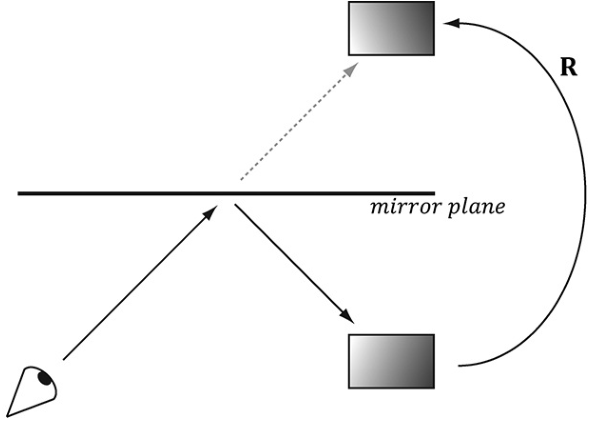
\includegraphics[width=\textwidth]{11-2}
    \centering
    \caption{眼睛通过镜子看到盒子反射。 为了模拟这一点,我们在镜像平面上将箱子反转并像往常一样渲染反转过的箱子。}
    \label{fig:11-2}
\end{figure}

\begin{figure}[h]
    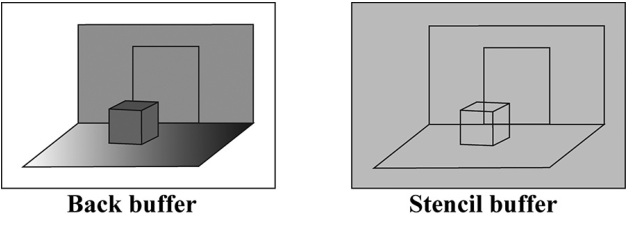
\includegraphics[width=\textwidth]{11-3}
    \centering
    \caption{后缓冲区和模板缓冲区的地板,墙壁和头骨清除为0(用浅灰色表示)。 模板缓冲区上绘制的黑色轮廓图示了后缓冲区像素和模板缓冲区像素之间的关系 - 它们不表示在模板缓冲区上绘制的任何数据。}
    \label{fig:11-3}
\end{figure}

\begin{flushleft}
1.将地板,墙壁和头骨渲染到后缓冲区进行普通渲染(不是镜像渲染)。 请注意,此步骤不会修改模板缓冲区。\\
2.将模板缓冲区清除为0.图\ref{fig:11-3}显示了此时的后缓冲区和模板缓冲区(颅骨用箱子代替)。\\
3.仅将镜像渲染到模板缓冲区。通过创建设置的混合状态来禁用对后台缓冲区的颜色写入\\
\end{flushleft}
\begin{lstlisting}
D3D12_RENDER_TARGET_BLEND_DESC::RenderTargetWriteMask = 0;
\end{lstlisting}
\begin{flushleft}
并且设置禁止写入到深度缓冲区\\
\end{flushleft}
\begin{lstlisting}
D3D12_DEPTH_STENCIL_DESC::DepthWriteMask = D3D12_DEPTH_WRITE_MASK_ZERO;
\end{lstlisting}
\begin{flushleft}
将镜像渲染到模板缓冲区时,将模板测试设置为始终成功(D3D12\_COMPARISON\_ALWAYS),并指定在测试通过时应将模板缓冲区条目替换为(SdcilRef)为 1(StencilRef)(D3D12\_STENCIL\_OP\_REPLACE)。如果深度测试失败,指定 D3D12\_STENCIL\_OP\_KEEP,以便在深度测试失败时不会更改模板缓冲区(例如,如果头骨遮挡了镜子的一部分,就会发生这种情况)。 由于我们只将镜像渲染到模板缓冲区,因此模板缓冲区中的所有像素都将为0,除了与镜像的可见部分对应的像素——它们的值为1。图\ref{fig:11-4}显示更新模板缓冲区。 基本上,在模板缓冲区中标记镜像的可见像素即可。
\end{flushleft}
\begin{figure}[h]
    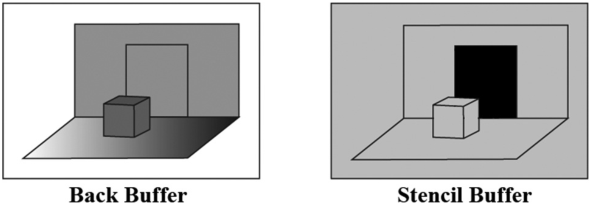
\includegraphics[width=\textwidth]{11-4}
    \centering
    \caption{将镜像渲染到模板缓冲区,实质上标记模板缓冲区中与镜像的可见部分对应的像素。 模板缓冲区上的实心黑色区域表示模板条目设置为1。请注意,模板缓冲区中箱子被遮挡的区域未设置为1,因为它未通过深度测试(箱子位于部分镜子的前面)。}
    \label{fig:11-4}
\end{figure}

\begin{flushleft}
~\\
NOTICE: 在绘制颅骨之后将镜像绘制到模板缓冲区是很重要的,这样颅骨遮挡的镜像不能通过深度测试,因此不会修改模板缓冲区。我们不想打开被遮挡的模板缓冲区的部分; 否则反射的头骨将通过正常头骨显示出来。
~\\
4.现在我们将反射的头骨渲染到后缓冲区和模板缓冲区。 但请记住,如果模板测试通过,只会渲染到后台缓冲区。 这次,将模板测试设置为仅在模板缓冲区中的值等于1时才成功; 这是使用StencilRef为1和模板操作符 D3D12\_COMPARISON\_EQUAL 完成的。 通过这种方式,反射的头骨将仅渲染到相应的模板缓冲区条目中具有1的区域。 由于模板缓冲区中与镜子的可见部分相对应的区域是唯一具有1的条目,因此反射的颅骨将仅被渲染到镜子的可见部分中。\\

5.最后,将镜像正常渲染到后缓冲区。 然而,为了显示反射的头骨(位于镜子后面),需要渲染具有透明度混合的镜子。 如果没有渲染具有透明度的镜子,镜子将简单地遮挡反射,因为它的深度小于反射的深度。 为了实现这一点,只需要为镜像定义一个新的材质实例; 我们将漫反射组件的alpha通道设置为0.3以使镜像30%不透明,并且我们使用透明度混合状态渲染镜像,如上一章(第10.5.4节)中所述。\\
\end{flushleft}

\begin{lstlisting}[escapechar=^]
auto icemirror = std::make_unique<Material>();
icemirror->Name = "icemirror";
icemirror->MatCBIndex = 2;
icemirror->DiffuseSrvHeapIndex = 2;
^\textbf{icemirror->DiffuseAlbedo = XMFLOAT4(1.0f, 1.0f, 1.0f, 0.3f);}^
icemirror->FresnelR0 = XMFLOAT3(0.1f, 0.1f, 0.1f);
icemirror->Roughness = 0.5f;
\end{lstlisting}

\begin{flushleft}
这些设置使用了混合公式:\\
\end{flushleft}

\begin{align*}
C=0.3\cdot C_{src}+0.7\cdot C_{dst}
\end{align*}

\begin{flushleft}
假设已经将反射的头骨像素放置到后缓冲区,我们看到30%的颜色来自镜子(源),70%的颜色来自头骨(目标)。
\end{flushleft}

%-------- 11.4.2 --------
\subsection{定义镜像的深度/模板状态(Defining the Mirror Depth/Stencil States)}
\begin{flushleft}
为了实现先前描述的算法,我们需要两个PSO。 第一个用于绘制镜像以标记模板缓冲区上的镜像像素。 第二个用于绘制反射的头骨,使其仅被吸入镜子的可见部分。\\
\end{flushleft}

\begin{lstlisting}[escapechar=^]
//
// PSO for marking stencil mirrors.
//

CD3DX12_BLEND_DESC mirrorBlendState(D3D12_DEFAULT);
^\textbf{mirrorBlendState.RenderTarget[0].RenderTargetWriteMask = 0;}^

D3D12_DEPTH_STENCIL_DESC mirrorDSS;
mirrorDSS.DepthEnable = true;
^\textbf{mirrorDSS.DepthWriteMask = D3D12_DEPTH_WRITE_MASK_ZERO;}^
mirrorDSS.DepthFunc = D3D12_COMPARISON_FUNC_LESS;
mirrorDSS.StencilEnable = true;
mirrorDSS.StencilReadMask = 0xff;
mirrorDSS.StencilWriteMask = 0xff;

mirrorDSS.FrontFace.StencilFailOp = D3D12_STENCIL_OP_KEEP;
^\textbf{mirrorDSS.FrontFace.StencilDepthFailOp = D3D12_STENCIL_OP_KEEP;}^
^\textbf{mirrorDSS.FrontFace.StencilPassOp = D3D12_STENCIL_OP_REPLACE;}^
^\textbf{mirrorDSS.FrontFace.StencilFunc = D3D12_COMPARISON_FUNC_ALWAYS;}^

// We are not rendering backfacing polygons, 
// so these settings do not matter.
mirrorDSS.BackFace.StencilFailOp = D3D12_STENCIL_OP_KEEP;
mirrorDSS.BackFace.StencilDepthFailOp = D3D12_STENCIL_OP_KEEP;
mirrorDSS.BackFace.StencilPassOp = D3D12_STENCIL_OP_REPLACE;
mirrorDSS.BackFace.StencilFunc = D3D12_COMPARISON_FUNC_ALWAYS;

D3D12_GRAPHICS_PIPELINE_STATE_DESC markMirrorsPsoDesc = opaquePsoDesc;
markMirrorsPsoDesc.BlendState = mirrorBlendState;
markMirrorsPsoDesc.DepthStencilState = mirrorDSS;
ThrowIfFailed(md3dDevice->CreateGraphicsPipelineState(
    &markMirrorsPsoDesc, 
    IID_PPV_ARGS(&mPSOs["markStencilMirrors"])));

//
// PSO for stencil reflections.
//

D3D12_DEPTH_STENCIL_DESC reflectionsDSS;
reflectionsDSS.DepthEnable = true;
reflectionsDSS.DepthWriteMask = D3D12_DEPTH_WRITE_MASK_ALL;
reflectionsDSS.DepthFunc = D3D12_COMPARISON_FUNC_LESS;
reflectionsDSS.StencilEnable = true;
reflectionsDSS.StencilReadMask = 0xff;
reflectionsDSS.StencilWriteMask = 0xff;

reflectionsDSS.FrontFace.StencilFailOp = D3D12_STENCIL_OP_KEEP;
reflectionsDSS.FrontFace.StencilDepthFailOp = D3D12_STENCIL_OP_KEEP;
reflectionsDSS.FrontFace.StencilPassOp = D3D12_STENCIL_OP_KEEP;
^\textbf{reflectionsDSS.FrontFace.StencilFunc = D3D12_COMPARISON_FUNC_EQUAL;}^

// We are not rendering backfacing polygons, 
// so these settings do not matter.
reflectionsDSS.BackFace.StencilFailOp = D3D12_STENCIL_OP_KEEP;
reflectionsDSS.BackFace.StencilDepthFailOp = D3D12_STENCIL_OP_KEEP;
reflectionsDSS.BackFace.StencilPassOp = D3D12_STENCIL_OP_KEEP;
reflectionsDSS.BackFace.StencilFunc = D3D12_COMPARISON_FUNC_EQUAL;

D3D12_GRAPHICS_PIPELINE_STATE_DESC drawReflectionsPsoDesc = opaquePsoDesc;
drawReflectionsPsoDesc.DepthStencilState = reflectionsDSS;
drawReflectionsPsoDesc.RasterizerState.CullMode = D3D12_CULL_MODE_BACK;
^\textbf{drawReflectionsPsoDesc.RasterizerState.FrontCounterClockwise = true;}^
ThrowIfFailed(md3dDevice->CreateGraphicsPipelineState(
    &drawReflectionsPsoDesc, 
    IID_PPV_ARGS(&mPSOs["drawStencilReflections"])));
\end{lstlisting}

%-------- 11.4.3 --------
\subsection{绘制场景(Drawing the Scene)}
\begin{flushleft}
以下代码概述了我们的绘制方法。 为简洁起见,省略了不相关的细节,例如设置常量缓冲区值(有关详细信息,请参阅示例代码)。
\end{flushleft}
\begin{lstlisting}
// Draw opaque items—floors, walls, skull.
auto passCB = mCurrFrameResource->PassCB->Resource();
mCommandList->SetGraphicsRootConstantBufferView(
    2,
    passCB->GetGPUVirtualAddress());
DrawRenderItems(
    mCommandList.Get(),
    mRitemLayer[(int)RenderLayer::Opaque]);
// Mark the visible mirror pixels in the stencil
buffer with the value 1
mCommandList->OMSetStencilRef(1);
mCommandList->SetPipelineState(
    mPSOs["markStencilMirrors"].Get());
DrawRenderItems(
    mCommandList.Get(),
    mRitemLayer[(int)RenderLayer::Mirrors]);
// Draw the reflection into the mirror only 
// (only for pixels where the stencil buffer is 1).
// Note that we must supply a different per-pass 
// constant buffer—one with the lights reflected.
mCommandList->SetGraphicsRootConstantBufferView(
    2,
    passCB->GetGPUVirtualAddress() + 1 * passCBByteSize);
mCommandList->SetPipelineState(
    mPSOs["drawStencilReflections"].Get());
DrawRenderItems(
    mCommandList.Get(),
    mRitemLayer[(int)RenderLayer::Reflected]);
// Restore main pass constants and stencil ref.
mCommandList->SetGraphicsRootConstantBufferView(2,
passCB->GetGPUVirtualAddress());
mCommandList->OMSetStencilRef(0);
// Draw mirror with transparency so reflection blends through.
mCommandList->SetPipelineState(mPSOs[“transparent”].Get());
DrawRenderItems(
    mCommandList.Get(),
    mRitemLayer[(int)RenderLayer::Transparent]);
\end{lstlisting}

\begin{flushleft}
在上面的代码中需要注意的一点是在绘制 RenderLayer::Reflected 图层时如何更改 per-pass 常量缓冲区。因为在绘制反射时场景时,照明也需要反射。 照明存储在 per-pass 常量缓冲区中,因此创建了一个额外的 per-pass 常量缓冲区,用于存储反射的场景照明。 用于绘制反射的 per-pass 常量缓冲区在以下方法中设置:\\
\end{flushleft}

\begin{lstlisting}
PassConstants StencilApp::mMainPassCB;
PassConstants StencilApp::mReflectedPassCB;
void StencilApp::UpdateReflectedPassCB(
    const GameTimer& gt)
{
    mReflectedPassCB = mMainPassCB;
    XMVECTOR mirrorPlane = XMVectorSet(0.0f, 0.0f, 1.0f, 0.0f); // xy plane
    XMMATRIX R = XMMatrixReflect(mirrorPlane);
    // Reflect the lighting.
    for(int i = 0; i < 3; ++i)
    {
        XMVECTOR lightDir =
        XMLoadFloat3(&mMainPassCB.Lights[i].Direction);
        XMVECTOR reflectedLightDir =
        XMVector3TransformNormal(lightDir, R);
        XMStoreFloat3(&mReflectedPassCB.Lights[i].Direction,
        reflectedLightDir);
    }
    // Reflected pass stored in index 1
    auto currPassCB = mCurrFrameResource->PassCB.get();
    currPassCB->CopyData(1, mReflectedPassCB);
}
\end{lstlisting}

%-------- 11.4.4 --------
\subsection{缠绕顺序和反射(Winding Order and Reflections)}
\begin{flushleft}
当三角形在平面上反射时,其定点的缠绕顺序不会反转,其面法线不会反转。 因此,在反射之后,朝外的法线变为了向内法线(见图\ref{fig:11-5})。 为了纠正这个问题,告诉Direct3D将逆时针缠绕顺序的三角形解释为面向前方,将三角形顺时针缠绕顺序解释为背面(这与惯例——5.10.2节相反)。 这能使法线方向也进行了反射,面朝向外。 通过在PSO中设置以下光栅化器属性来反转绕线顺序约定:\\
\end{flushleft}

\begin{lstlisting}
drawReflectionsPsoDesc.RasterizerState.FrontCounterClockwise = true;
\end{lstlisting}

\begin{figure}[h]
    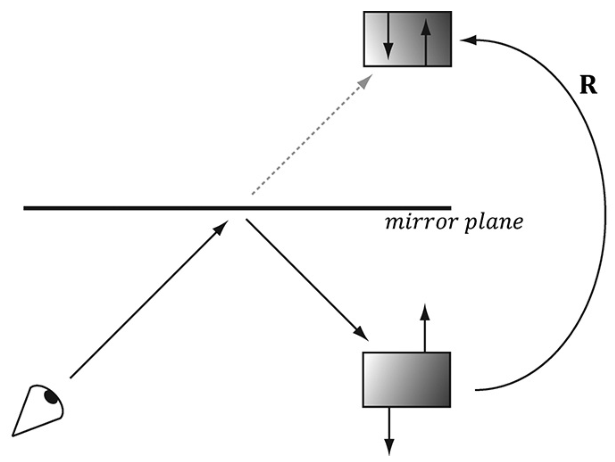
\includegraphics[width=\textwidth]{11-5}
    \centering
    \caption{多边形法线不会被反射反转,这使得它们在反射后,面朝向内。}
    \label{fig:11-5}
\end{figure}

%-------- 11.5 --------
\section{实现平面阴影(Implementing Planar Shadows)}
\begin{flushleft}
~\\
NOTICE: 本节的部分内容出现在Frank D. Luna的书中,DirectX 9.0c的3D游戏编程简介:Shader Approach,2006:Jones和Bartlett Learning,Burlington,MA。www.jblearning.com。 经许可重印。
~\\

阴影有助于我们了解场景中光线的发射位置,并最终使场景更加逼真。 在本节中,我们将展示如何实现平面阴影;(见图\ref{11-6})。\\
\end{flushleft}

\begin{figure}[h]
    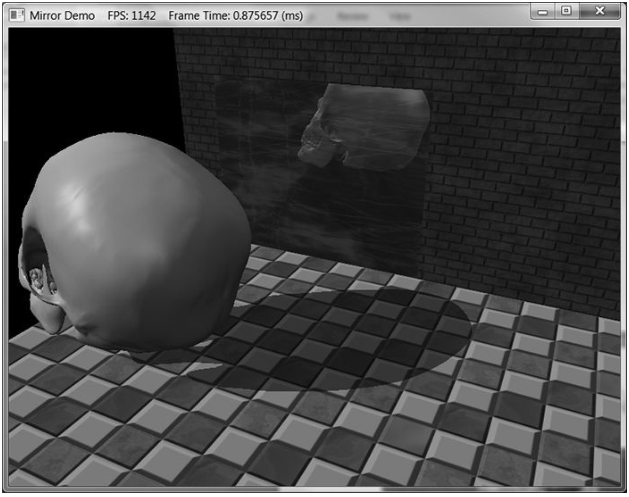
\includegraphics[width=\textwidth]{11-6}
    \centering
    \caption{主光源在“镜子”演示中投射了一个平面阴影。}
    \label{fig:11-6}
\end{figure}

\begin{flushleft}
要实现平面阴影,必须首先找到对象投射到平面的阴影并对其进行几何建模。 这可以通过一些3D数学轻松完成。 然后,使用50%透明度的黑色材质渲染描述阴影的三角形。 像这样渲染阴影会引入一些称为“双重混合”的渲染物体,我们将在几个部分中进行解释; 利用模板缓冲区来防止发生双重混合。\\
\end{flushleft}

\begin{figure}[h]
    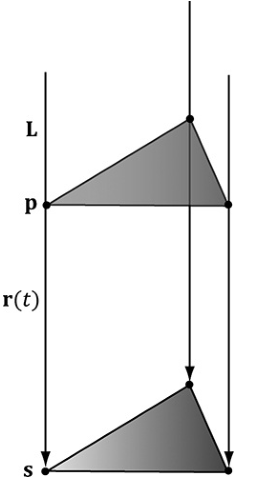
\includegraphics[width=\textwidth]{11-7}
    \centering
    \caption{相对于平行光源投射的阴影。}
    \label{fig:11-7}
\end{figure}

%-------- 11.5.1 --------
\subsection{平行光源阴影(Parallel Light Shadows)}
\begin{flushleft}
图\ref{fig:11-7}显示了一个物体相对于平行光源投射的阴影。 给定方向$L$的平行光源,穿过顶点$p$的光线由$r(t)=\boldsymbol{p}+t\boldsymbol{L}$给出。 光线$r(t)$与阴影平面$(\boldsymbol{n},d)的交点给出$\boldsymbol{s}$。 (读者可以在附录C中阅读有关光线和平面的更多信息。)通过使用平面拍摄穿过每个物体顶点的光线而得到的交叉点集定义了阴影的投影几何形状。 对于顶点$\boldsymbol{p}$,其阴影投影由下式给出\\
\end{flushleft}

\begin{align*}\tag{eq.11.1}\label{eq.11.1}
s=r(t_{s})=\boldsymbol{p}-\frac{\boldsymbol{n}\cdot \boldsymbol{p}+d}{\boldsymbol{n}\cdot \boldsymbol{L}}\boldsymbol{L}
\end{align*}

\begin{flushleft}
射线/平面相交测试的细节在附录C中给出。\\
公式\ref{eq.11.1}可以用矩阵编写。\\
\end{flushleft}

\begin{align*}
s^{'}=\begin{bmatrix}
p_{x} & p_{y} & p_{z} & 1
\end{bmatrix}
\begin{bmatrix}
\boldsymbol{n}\cdot \boldsymbol{L}-L_{x}n_{x} & -L_{y}n_{x} & -L_{z}n_{x} & 0\\
-L_{x}n_{y} & \boldsymbol{n}\cdot \boldsymbol{L}-L_{y}n_{y} & -L_{z}n_{y} & 0\\
-L_{x}n_{z} & -L_{y}n_{z} & \boldsymbol{n}\cdot \boldsymbol{L}-L_{z}n_{z} & 0\\
-L_{x}d & -L_{y}d & -L_{z}d & \boldsymbol{n}\cdot \boldsymbol{L}
\end{bmatrix}
\end{align*}

\begin{flushleft}
我们将前面的$4\times 4$矩阵称为方向阴影矩阵,并用$S_{dir}$表示。 要了解此矩阵如何等效于公式\ref{eq.11.1},只需要执行乘法运算。 然而,首先,观察该等式修改$w$分量,使得$s_{w}=\boldsymbol{n}\cdot \boldsymbol{L}$。 因此,当发生透视分割(5.6.3.4节)时,$s$的每个坐标将除以$\boldsymbol{n}\cdot \boldsymbol{L}$; 这就是我们如何使用矩阵得到公式\ref{eq.11.1}中$\boldsymbol{n}\cdot \boldsymbol{L}$的除法。 现在进行矩阵乘法以获得$i\epsilon {1,2,3}$的第$i$个坐标$s^{'}_{i}$,然后是我们获得的透视除法:\\
\end{flushleft}

\begin{align*}
s^{'}_{i}&=\frac{(\boldsymbol{n}\cdot \boldsymbol{L})p_{i}-L_{i}n_{x}p_{x}-L_{i}n_{y}p_{y}-L_{i}n_{z}p_{z}-L_{i}d)}{\boldsymbol{n}\cdot \boldsymbol{L}}\\
&=\frac{(\boldsymbol{n}\cdot \boldsymbol{L})p_{i}-(\boldsymbol{n}\cdot \boldsymbol{p}+d)L_{i}}{\boldsymbol{n}\cdot \boldsymbol{L}}\\
&=p_{i}-\frac{\boldsymbol{n}\cdot \boldsymbol{p}+d}{\boldsymbol{n}\cdot \boldsymbol{L}}L_{i}
\end{align*}

\begin{flushleft}
这正是公式\ref{eq.11.1}中$\boldsymbol{s}$的第$i$个坐标,所以$\boldsymbol{s}=\boldsymbol{s^{'}}$。\\

要使用阴影矩阵,将它与我们的世界矩阵相结合。 在世界变换之后,几何体还没有真正投射到阴影平面上,因为尚未发生透视分割。如果$s_{w}=n\cdot L<0$则会出现问题,因为这使得$w$坐标为负。 通常在透视投影过程中,将$z$坐标复制到$w$坐标,负$w$坐标意味着该点不在视图体积中,因此被剪掉(剪切在划分之前在齐次空间中完成)。 这是平面阴影的问题,因为除了透视分割之外,我们现在使用$w$坐标来实现阴影。 图\ref{fig:11-8}显示了一个有效的情况,其中$n\cdot L<0$,但阴影不会显示。\\
\end{flushleft}

\begin{figure}[h]
    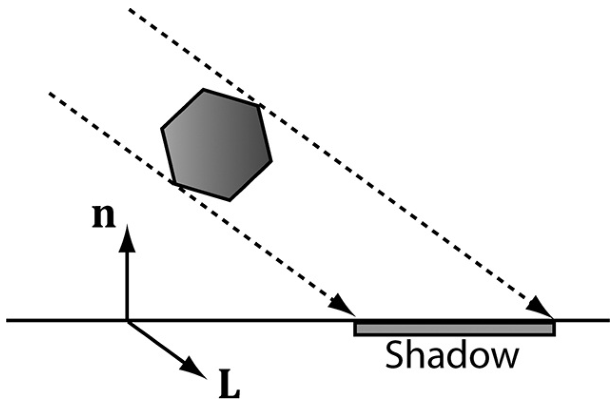
\includegraphics[width=\textwidth]{11-8}
    \centering
    \caption{$n\cdot L<0$的情况。}
    \label{fig:11-8}
\end{figure}

\begin{flushleft}
为了解决这个问题,我们应该使用向量朝向无限远的光源$L^{\infty}=-L$替换定向光源$L$。 观察$r(t)=p+tL$和$r(t)=p+tL^{\infty}$定义相同的3D线,并且线与平面之间的交点是相同的(为了补偿$L^{\infty}$和$L$之间的符号差异,交点参数$t_{s}$将变得不同)。使用$L^{\infty}=-L$给出了相同的答案,$n\cdot L>0$,这避免了负$w$坐标。\\
\end{flushleft}

%-------- 11.5.2 --------
\subsection{点光源阴影(Point Light Shadows)}
\begin{figure}[h]
    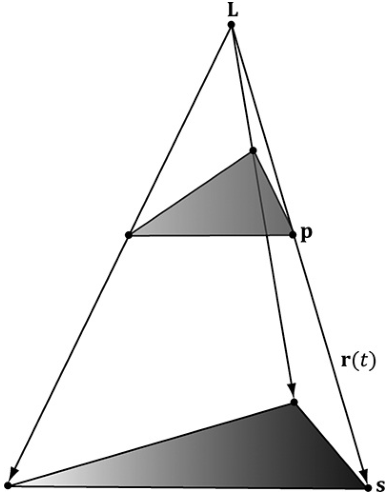
\includegraphics[width=\textwidth]{11-9}
    \centering
    \caption{相对于点光源投射的阴影。}
    \label{fig:11-9}
\end{figure}

\begin{flushleft}
图\ref{fig:11-9}显示了一个物体相对于点光源投射的阴影,其点位置由点$L$描述。点光源通过任何顶点$p$的光线由$r(t)=p+t(p-L)$给出)。 光线$r(t)$与阴影平面$(n,d)$的交点给出$s$。 射线穿过每个物体顶点与平面相交的点集定义了阴影的投影几何形状。对于顶点$p$,其阴影投影由下式给出\\
\end{flushleft}

\begin{align*}\tag{eq.11.2}\label{eq.11.2}
s=r(t_{s})=p-\frac{n\cdot p+d}{n\cdot (p-L)}(p-L)
\end{align*}

\begin{flushleft}
公式\ref{eq.11.2}能携程矩阵形式:\\
\end{flushleft}

\begin{align*}
S_{point}=\begin{bmatrix}
 n\cdot L+d-L_{x}n_{x} & -L_{y}n_{x} & -L_{z}n_{x} & -n_{x} \\
 -L_{x}n_{y} & n\cdot L+d-L_{y}n_{y} & -L_{z}n_{y} & -n_{y} \\
 -L_{x}n_{z} & -L_{y}n_{z} & n\cdot L+d-L_{z}n_{z} & -n_{z} \\
 -L_{x}d & -L_{y}d & -L_{z}d & n\cdot L
\end{bmatrix}
\end{align*}

\begin{flushleft}
要了解此矩阵如何等效于公式\ref{eq.11.2},我们只需要像上一节中那样执行乘法。 请注意,最后一列没有零:\\
\end{flushleft}

\begin{align*}
s_{w}&=-p_{x}n_{x}-p_{y}n_{y}-p_{z}n_{z}+n\cdot L\\
&=-p\cdot n+n\cdot L\\
&=-n\cdot (p-L)
\end{align*}

\begin{flushleft}
这是公式\ref{eq.11.2}中分母的负数,但如果我们使分子变负数,就可以使分母变负。\\

~\\
NOTICE: 请注意,$L$为点和平行光源提供不同的用途。 对于点光源,我们使用$L$来定义点光源的位置。 对于平行光,我们使用$L$来定义朝向无限远光源的方向(即,平行光线行进的相反方向)。
~\\
\end{flushleft}

%-------- 11.5.3 --------
\subsection{一般阴影矩阵(General Shadow Matrix)}
\begin{flushleft}
使用齐次坐标,可以创建一个适用于点光源和定向光源的通用阴影矩阵。\\

1.如果$L_{w}=0$则$L$表示朝向无限远光源的方向(即,平行光线行进的方向相反)。\\
2.如果$L_{w}=1$,则$L$描述点光源的位置。\\

用以下阴影矩阵表示从顶点$p$到其投影$s$的变换:\\
\end{flushleft}

\begin{align*}
\boldsymbol{S}=\begin{bmatrix}
 n\cdot L+dL_{w}-L_{x}n_{x} & -L_{y}n_{x} & -L_{z}n_{x} & -L_{w}n_{x} \\
 -L_{x}n_{y} & n\cdot L+dL_{w}-L_{y}n_{y} & -L_{z}n_{y} & -L_{w}n_{y} \\
 -L_{x}n_{z} & -L_{y}n_{z} & n\cdot L+dL_{w}-L_{z}n_{z} & -L_{w}n_{z} \\
 -L_{x}d & -L_{y}d & -L_{z}d & n\cdot L
\end{bmatrix}
\end{align*}

\begin{flushleft}
不难看出如果$L_{w}=0$则$S$会减小到$S_{dir}$;如果 $L_{w}=1$,则$S$会减小到$S_{point}$,则。\\

给定我们希望投影阴影的平面,以及如果$w=0$则是描述平行光的向量或者如果$w=1$,则为点光源,DirectX数学库提供以下函数来构建阴影矩阵:\\
\end{flushleft}

\begin{lstlisting}
inline XMMATRIX XM_CALLCONV XMMatrixShadow(
    FXMVECTOR ShadowPlane,
    FXMVECTOR LightPosition);
\end{lstlisting}

\begin{flushleft}
先要了解更多,[Blinn96] 和 [Möller02] 都讨论了平面阴影。
\end{flushleft}

%-------- 11.5.4 --------
\subsection{使用模板缓冲区防止双混合(Using the Stencil Buffer to Prevent Double Blending)}
\begin{flushleft}
当我们将对象的几何形状展铺到平面上以描述其阴影时,可能(并且实际上可能)两个或更多个展平的三角形重叠。 当使用透明度渲染阴影时(使用混合),具有重叠三角形的这些区域将多次混合,显得更暗。 图\ref{fig:11-10}显示了这一点。\\
\end{flushleft}

\begin{figure}[h]
    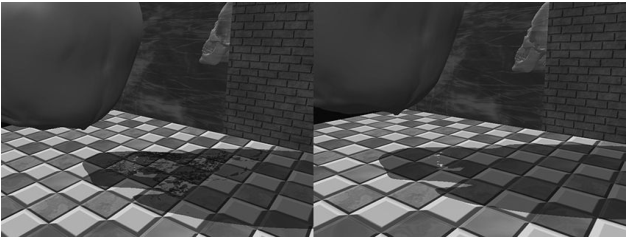
\includegraphics[width=\textwidth]{11-10}
    \centering
    \caption{注意左图中阴影的较暗“痤疮”区域; 这些对应于扁平颅骨部分重叠的区域,导致“双重混合”。右侧的图像显示正确渲染的阴影,没有双重混合。}
    \label{fig:11-10}
\end{figure}

\begin{flushleft}
我们能使用模板缓冲区解决这个问题:\\
1.假设将渲染阴影的模板缓冲区像素清除为0。在镜像演示中也是如此,因为我们只是在地平面上投射阴影,并且只修改了镜像模板缓冲区像素。\\
2.如果模板缓冲区的条目为0,则将模板测试设置为仅接受像素。如果模板测试通过,则我们将模板缓冲区值增加到1。\\

第一次渲染阴影像素时,模板测试将通过,因为模板缓冲区条目为0.但是,当我们渲染此像素时,我们还将相应的模板缓冲区条目递增为1.因此,如果我们尝试覆盖到 已经渲染到的区域(在模板缓冲区中标记值为1),模板测试将失败。 这可以防止在同一像素上多次绘制,从而防止双重混合。\\
\end{flushleft}


%-------- 11.5.5 --------
\subsection{阴影代码(Shadow Code)}
\begin{flushleft}
我们定义了一个用于为阴影着色的阴影材质,它只是50%透明的黑色材质:\\
\end{flushleft}

\begin{lstlisting}
auto shadowMat = std::make_unique<Material>();
shadowMat->Name = "shadowMat";
shadowMat->MatCBIndex = 4;
shadowMat->DiffuseSrvHeapIndex = 3;
shadowMat->DiffuseAlbedo = XMFLOAT4(0.0f, 0.0f, 0.0f, 0.5f);
shadowMat->FresnelR0 = XMFLOAT3(0.001f, 0.001f, 0.001f);
shadowMat->Roughness = 0.0f;
\end{lstlisting}

\begin{flushleft}
为了防止双重混合,我们设置了具有深度/模板状态的以下PSO:\\
\end{flushleft}

\begin{lstlisting}[escapechar=^]
// We are going to draw shadows with transparency, 
// so base it off the transparency description.
D3D12_DEPTH_STENCIL_DESC shadowDSS;
shadowDSS.DepthEnable = true;
shadowDSS.DepthWriteMask = D3D12_DEPTH_WRITE_MASK_ALL;
shadowDSS.DepthFunc = D3D12_COMPARISON_FUNC_LESS;
shadowDSS.StencilEnable = true;
shadowDSS.StencilReadMask = 0xff;
shadowDSS.StencilWriteMask = 0xff;

shadowDSS.FrontFace.StencilFailOp = D3D12_STENCIL_OP_KEEP;
shadowDSS.FrontFace.StencilDepthFailOp = D3D12_STENCIL_OP_KEEP;
^\textbf{shadowDSS.FrontFace.StencilPassOp = D3D12_STENCIL_OP_INCR;}^
^\textbf{shadowDSS.FrontFace.StencilFunc = D3D12_COMPARISON_FUNC_EQUAL;}^

// We are not rendering backfacing polygons, 
// so these settings do not matter.
shadowDSS.BackFace.StencilFailOp = D3D12_STENCIL_OP_KEEP;
shadowDSS.BackFace.StencilDepthFailOp = D3D12_STENCIL_OP_KEEP;
shadowDSS.BackFace.StencilPassOp = D3D12_STENCIL_OP_INCR;
shadowDSS.BackFace.StencilFunc = D3D12_COMPARISON_FUNC_EQUAL;

D3D12_GRAPHICS_PIPELINE_STATE_DESC shadowPsoDesc = transparentPsoDesc;
shadowPsoDesc.DepthStencilState = shadowDSS;
ThrowIfFailed(md3dDevice->CreateGraphicsPipelineState(
    &shadowPsoDesc, 
    IID_PPV_ARGS(&mPSOs["shadow"])));
\end{lstlisting}

\begin{flushleft}
然后,我们使用阴影PSO绘制头骨阴影,StencilRef值为0:\\
\end{flushleft}

\begin{lstlisting}
// Draw shadows
mCommandList->OMSetStencilRef(0);
mCommandList->SetPipelineState(mPSOs["shadow"].Get());
DrawRenderItems(
    mCommandList.Get(),
    mRitemLayer[(int)RenderLayer::Shadow]);
\end{lstlisting}
\begin{flushleft}
头骨阴影渲染项的世界矩阵如下:\\
\end{flushleft}

\begin{lstlisting}
// Update shadow world matrix.
XMVECTOR shadowPlane = XMVectorSet(0.0f, 1.0f, 0.0f, 0.0f); // xz plane
XMVECTOR toMainLight = -XMLoadFloat3(&mMainPassCB.Lights[0].Direction);
XMMATRIX S = XMMatrixShadow(shadowPlane, toMainLight);
XMMATRIX shadowOffsetY = XMMatrixTranslation(0.0f, 0.001f, 0.0f);
XMStoreFloat4x4(
    &mShadowedSkullRitem->World,
    skullWorld * S * shadowOffsetY);
\end{lstlisting}

\begin{flushleft}
请注意,我们沿$y$轴偏移投影的阴影网格很少以防止z-fighting,因此阴影网格不会与地板网格相交,而是略微位于其上方。 如果网格确实相交,那么由于深度缓冲区的精度有限,我们会看到闪烁的瑕疵,因为地板和阴影网格像素竞争可见。
\end{flushleft}

%-------- 11.6 --------
\section{总结}
\begin{flushleft}
1.模板缓冲区是一个屏幕外缓冲区,我们可以用来阻止某些像素片段渲染到后台缓冲区。 模板缓冲区与深度缓冲区共享,因此具有与深度缓冲区相同的分辨率。有效的深度/模板缓冲区格式为 DXGI\_FORMAT\_D32\_FLOAT\_S8X24\_UINT 和 DXGI\_FORMAT\_D24\_UNORM\_S8\_UINT。\\

2.防止特定像素被写入由模板测试决定,模板测试由以下内容给出:\\
\end{flushleft}

\begin{align*}
if(StencilRef 
   & StencilReadMask Value 
   & StencilReadMask )
    accept pixel
else
    reject pixel
\end{align*}

\begin{flushleft}
3.其中$\unlhd$运算符是 D3D12\_COMPARISON\_FUNC 枚举类型中定义的任何一个函数。 StencilRef,StencilReadMask,StencilReadMask 和比较运算符$\unlhd$都是使用Direct3D深度/模板API设置的应用程序定义的数量集合。其值数量是模板缓冲区中的当前值。\\
4.深度/模板状态是PSO描述的一部分。具体来说,通过填写 D3D12\_GRAPHICS\_PIPELINE\_STATE\_DESC::DepthStencilState 字段来配置深度/模板状态,其中 DepthStencilState 的类型为 D3D12\_DEPTH\_STENCIL\_DESC。\\
5.模板参考值使用 ID3D12GraphicsCommandList::OMSetStencilRef 方法设置,该方法采用指定模板参考值的单个无符号整数参数。\\
\end{flushleft}


%-------- 11.7 --------
\section{练习}
\begin{flushleft}
1.证明当 $L_{w}=0$时,一般阴影矩阵$S$缩减为$S_{dir}$,当$L_{w}=1$时,$S$缩减为$S_{point}$\\
2.证明 $s=p-\frac{n\cdot p+d}{n\cdot (p-L)}(p-L)=pS_{point}$,通过对每个分量进行矩阵乘法,如11.5.1中针对定向灯所做的那样。\\
3.修改“镜像”演示,生成图\ref{fig:11-1}中的“左”图像。\\
4.修改“镜像”演示,生成图\ref{fig:11-10}中的“左”图像。\\
5.修改“镜像”演示。首先用下面的深度设置绘制一堵墙:\\
\end{flushleft}

\begin{lstlisting}
depthStencilDesc.DepthEnable = false;
depthStencilDesc.DepthWriteMask = D3D12_DEPTH_WRITE_MASK_ALL;
depthStencilDesc.DepthFunc = D3D12_COMPARISON_LESS;
\end{lstlisting}

\begin{flushleft}
接着,在墙后面用下面深度设置绘制头骨:\\
\end{flushleft}

\begin{lstlisting}
depthStencilDesc.DepthEnable = true;
depthStencilDesc.DepthWriteMask = D3D12_DEPTH_WRITE_MASK_ALL;
depthStencilDesc.DepthFunc = D3D12_COMPARISON_LESS;
\end{lstlisting}

\begin{flushleft}
墙是否遮挡了头骨?请说明原因。如果您使用以下方法来绘制墙壁会发生什么?\\
\end{flushleft}

\begin{lstlisting}
depthStencilDesc.DepthEnable = true;
depthStencilDesc.DepthWriteMask = D3D12_DEPTH_WRITE_MASK_ALL;
depthStencilDesc.DepthFunc = D3D12_COMPARISON_LESS;
\end{lstlisting}

\begin{flushleft}
请注意,此练习不使用模板缓冲区,应在该练习中禁用模板缓冲区。\\

6.修改“镜像”演示,不反转三角形绕线顺序。反射的茶壶是否正确渲染?\\
7.修改第10章中的“Blend”演示,在场景的中心绘制一个圆柱体(没有帽子)。 使用加法混合在本章的目录中找到60帧动画电子螺栓动画来构造圆柱体。效果如图\ref{fig:11-11}。\\
\end{flushleft}

\begin{figure}[h]
    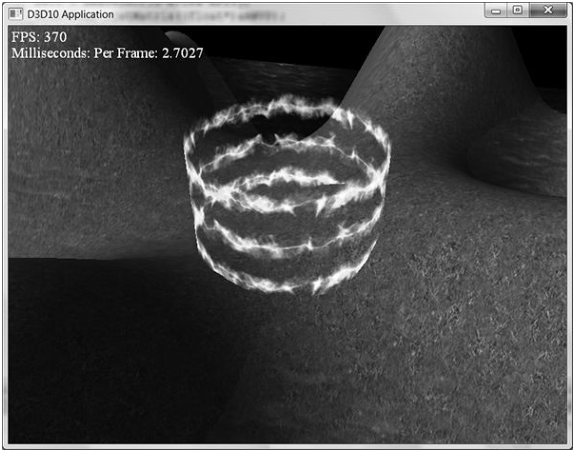
\includegraphics[width=\textwidth]{11-11}
    \centering
    \caption{练习7的效果截图}
    \label{fig:11-11}
\end{figure}

\begin{flushleft}
8.深度复杂度是指通过深度测试竞争写入后缓冲器中的特定条目的像素片段的数量。 例如,我们绘制的像素可能被更接近相机的像素覆盖(并且在绘制整个场景后实际计算出最近的像素之前,这可能会发生几次)。 图\ref{fig:11-12}中的像素的深度复杂度为3,因为三个像素片段竞争像素。
\end{flushleft}

\begin{figure}[h]
    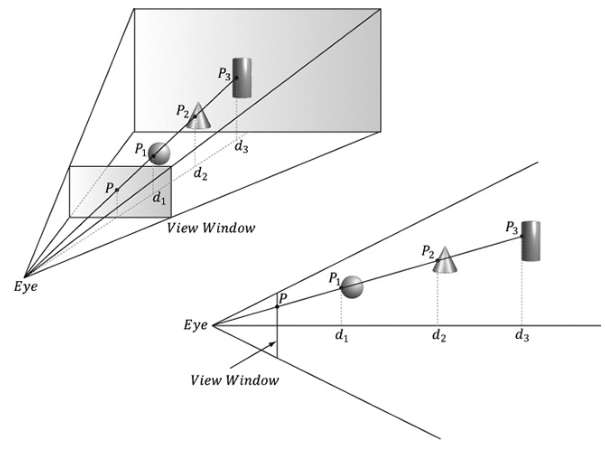
\includegraphics[width=\textwidth]{11-12}
    \centering
    \caption{多个像素片段竞争渲染到投影窗口上的单个像素。在该场景中,像素P的深度复杂度为3。}
    \label{fig:11-12}
\end{figure}

\begin{flushleft}
可能,显卡每帧可以填充几次像素。 这种过度绘制会影响性能,因为显卡浪费时间处理这些像素,最终被覆盖。 所以,测量场景中的深度复杂度以进行性能分析是有用的。\\

我们能以如下方式测量深度复杂度:渲染场景并使用模板缓冲区作为计数器; 也就是说,模板缓冲区中的每个像素最初都被清零,每次处理像素片段时,我们都会用 D3D12\_STENCIL\_OP\_INCR 递增计数。使用模板比较函数 D3D12\_COMPARISON\_ALWAYS,对应的模板缓冲区条目会始终为每个像素片段递增。 然后,例如,在绘制帧之后,如果第$i$个像素在模板缓冲区中具有相应的五个条目,则知道在该帧期间针对该像素处理了五个像素片段(即,像素深度复杂度为五)。 请注意,在计算深度复杂度时,从技术上讲,您只需要将场景渲染到模板缓冲区即可。\\

要可视化深度复杂度(存储在模板缓冲区中),请执行以下操作:\\

1.为每个深度复杂度$k$关联颜色$c_{k}$。 例如,蓝色表示深度复杂度为$1$,绿色表示深度复杂度为$2$,红色表示深度复杂度为$3$,依此类推。 (在非常复杂的场景中,像素的深度复杂度会变得非常大,您可能不希望为每个级别关联一种颜色。相反,您可以将颜色与一段连续的复杂度关联。例如,具有深度的像素复杂度1-5为蓝色,深度复杂度为6-10的像素为绿色,依此类推。)\\

2.将模板缓冲区操作符设置为 D3D12\_STENCIL\_OP\_KEEP,不再修改它。 (当我们在渲染场景,计算深度复杂度时,用 D3D12\_STENCIL\_OP\_INCR 修改模板缓冲区,但是当编写代码来可视化模板缓冲区时,我们只需要从模板缓冲区读取,我们不应该写入它。)\\

3.对于每个深度复杂度$k$级:\\
\end{flushleft}

\begin{itemize}
  \item (1).将模板比较功能设置为 D3D12\_COMPARISON\_EQUAL,并将模板参考值设置为$k$。
  \item (2).绘制覆盖整个投影窗口的四边形颜色$c_{k}$。 请注意,由于前面的模板比较功能和参考值,这只会对深度复杂度为$k$的像素进行着色。
\end{itemize}

\begin{flushleft}
通过这种设置,我们可以根据其深度复杂度对每个像素进行唯一着色,因此我们可以轻松地研究场景的深度复杂性。 在本练习中,渲染第10章“Blend”演示中使用的场景的深度复杂度。图\ref{fig:11-13}显示了一个示例屏幕截图。
\end{flushleft}

\begin{figure}[h]
    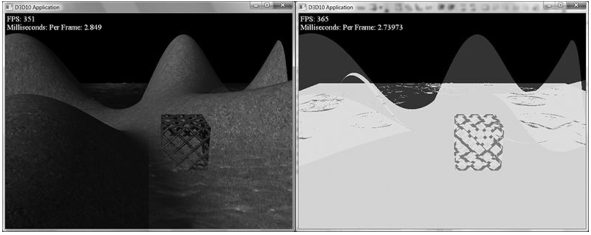
\includegraphics[width=\textwidth]{11-13}
    \centering
    \caption{练习8的截图}
    \label{fig:11-13}
\end{figure}

\begin{flushleft}
~\\
NOTICE:深度测试发生在管道的输出合并阶段,该阶段发生在像素着色器阶段之后。这意味着即使最终可能被深度测试拒绝,也会经过像素着色器处理像素片段。现代硬件会进行“early z-test”,这会在像素着色器之前执行深度测试。这样,被丢弃的像素片段在可能被昂贵的像素着色器处理之前被丢弃。要利用此优化,您应该尝试相对于相机以前后顺序渲染非混合游戏对象;首先绘制最近的对象,它们后面的对象就会无法通过early z-test而不会被进一步处理。如果由于高深度复杂性而导致场景遭受大量过度绘制的情况,使用 early z-test 会带来显着的性能优势。我们无法通过Direct3D API控制early z-test;是否可以执行early z-test由图形驱动程序决定。例如,如果像素着色器会修改像素片段的深度值,则不可能进行early z-test,因为像素着色器必须在深度测试之前执行。
~\\
NOTICE: 我们提到了修改像素着色器中像素深度的功能。这是如何运作的? 像素着色器实际上可以输出结构体,而不仅仅是我们到目前为止所做的单个颜色向量:\\
\end{flushleft}

\begin{lstlisting}
struct PixelOut
{
    float4 color : SV_Target;
    float depth : SV_Depth;
};
PixelOut PS(VertexOut pin)
{
    PixelOut pout;
    // ...usual pixel work
    pout.Color = float4(litColor, alpha);
    // set pixel depth in normalized [0, 1] range
    pout.depth = pin.PosH.z - 0.05f;
    return pout;
}
\end{lstlisting}

\begin{flushleft}
SV\_Position 元素的 z坐标(pin.PosH.z)给出未修改的像素深度值。使用特殊系统值语义 SV\_Depth,像素着色器可以输出修改的深度值。\\
~\\
9.实现深度复杂性可视化的另一种方法是使用加法混合。首先清除后面的缓冲区黑色并禁用深度测试。接下来,将源和目标混合因子都设置为 D3D12\_BLEND\_ONE,将混合操作设置为 D3D12\_BLEND\_OP\_ADD,以使混合方程看起来像 $C=C_{src}+C_{dst}$。观察这个公式,对于每个像素,累加写入它的所有像素片段的颜色。现在使用像素着色器渲染场景中的所有对象,该像素着色器输出低强度颜色,如$(0.05,0.05,0.05)$。一个像素越多的过度绘制,这些低强度颜色累加,增加了亮度。例如,如果一个像素过度绘制了十次,那么它的颜色强度将为$(0.5,0.5,0.5)$。因此,在渲染场景之后每个像素的强度显示了该像素的深度复杂度。使用第10章中的“Blend”演示作为测试场景,实现此版本的深度复杂度测量。\\

10.解释如何计算通过深度测试的像素数。解释如何计算未通过深度测试的像素数?\\
11.修改“镜子”演示,除头骨之外在镜子中对地面做镜面反射。\\
12.从阴影渲染项的世界矩阵中删除垂直偏移量,以便您可以看到 z-fighting 现象。\\
\end{flushleft}
